\begin{frame}
\frametitle{Классы памяти}

\onslide<1->{По привилегиям доступа:
\begin{enumerate}
  \item привилегированная (kernel space)
  \item не привилегированная (user space)
\end{enumerate}}

\onslide<2->{По способу аллокации:
\begin{enumerate}
  \item статическая память (код, глобальные переменные - размер известен заранее)
  \item динамическая память (куча, free store и тд - размер не известен заранее)
\end{enumerate}}
\end{frame}

\begin{frame}
\frametitle{Карта памяти}

\begin{columns}[T]

  \begin{column}{.4\textwidth}
    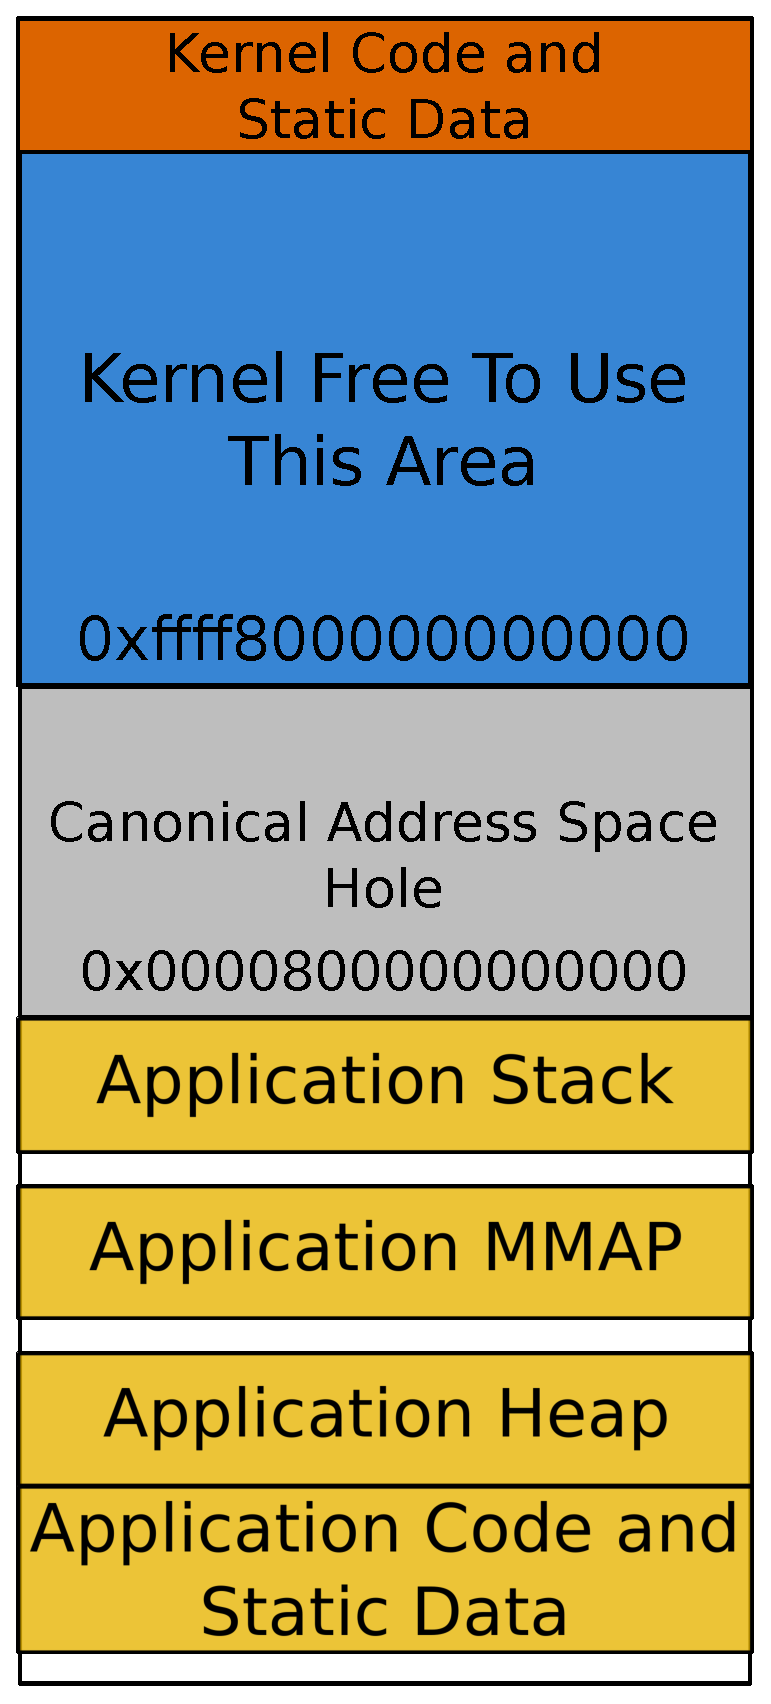
\includegraphics[width=.8\linewidth]{memmap}
  \end{column}

  \begin{column}{.6\textwidth}
    \begin{itemize}
      \item Kernel Code and Static Data - привилегированная статическая память (System V ABI amd64, 3.5.1 Architectural Constraints, Kernel code model)
      \item Canonical Address Space Hole - недопустимые адреса памяти (Intel\textsuperscript{\textregistered} 64 and IA-32 Architectures Software Developer's Manual, 3.3.7.1 Canonical Addressing)
    \end{itemize}
  \end{column}
\end{columns}

\end{frame}

\begin{frame}
\frametitle{Карта памяти}

\begin{columns}[T]

  \begin{column}{.4\textwidth}
    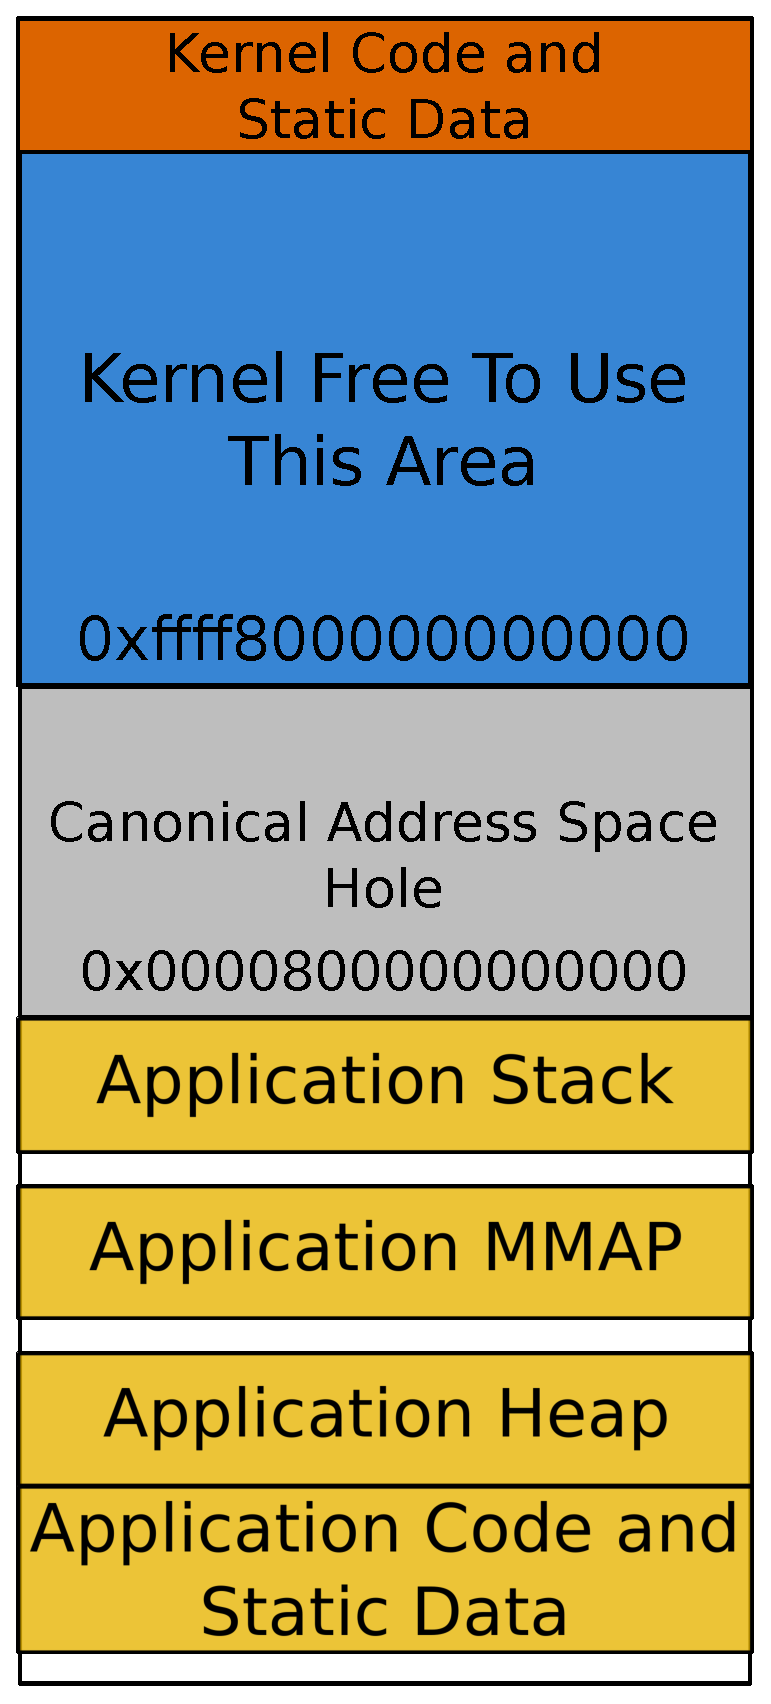
\includegraphics[width=.8\linewidth]{memmap}
  \end{column}

  \begin{column}{.6\textwidth}
    \begin{itemize}
      \item Application Stack - аллоцируется ОС при старте программы
      \item Application MMAP - разделяемые библиотеки, mmap/munmap
      \item Application Heap - malloc берет память отсюда, изменяется системным вызовом sbrk
      \item Application Code and Static Data - статическая не привилегированная память
    \end{itemize}
  \end{column}
\end{columns}

\end{frame}

